\documentclass[14pt,a4paper]{report}

\usepackage{cmap}
\usepackage[warn]{mathtext}
\usepackage[utf8x]{inputenc}
\usepackage[T1,T2A]{fontenc}
\usepackage[english,russian]{babel}
\usepackage{indentfirst}
\usepackage{amsmath}
\usepackage{amsfonts}
\usepackage{amssymb}
\usepackage{graphicx}
\graphicspath{{image/}}
\usepackage{listings}
\usepackage{hyperref}
\usepackage{float}
\usepackage{fontspec}
\usepackage{placeins}
\setmainfont{SFNS Display}
\setmonofont{SFNS Display}

\lstset{
	inputencoding=utf8x,
	extendedchars=\true,
	frame=single,
	breaklines=true,
	numbers=left,
	keepspaces = true}

\voffset -24.5mm
\hoffset -5mm
\textwidth 173mm
\textheight 240mm
\oddsidemargin=0mm \evensidemargin=0mm


\begin{document}
	\begin{titlepage}
\begin{center}

\textbf{Санкт-Петербургский политехнический университет Петра Великого}

\vspace{5mm}
Институт компьютерных наук и технологий

\vspace{5mm}
Кафедра компьютерных систем и программных технологий

\vspace*{\fill}

\huge{Курсовой проект}

%\Large{о лабораторной работе №1}

\large{по дисциплине: <<Проектирование операционных систем>>}

\vspace*{2mm}
\large{Тема: <<Разработка демона звонков>>}

\vspace*{\fill}
\end{center}

%\begin{flushright}
\begin{large}
\hspace{0.4\linewidth} \textbf{Работу выполнил студент}

\vspace{5mm}
\hspace{0.4\linewidth} 13541/4 \hspace{1cm} \textit{Зорин А. Г.}

\vspace{3mm}
\hspace{0.4\linewidth} \textbf{Преподаватель}

\vspace{5mm}
\hspace{0.4\linewidth} \underline{\hspace{2cm} } \hspace{3mm} \textit{Душутина Е.В.}
\end{large}
%\end{flushright}

\vspace*{3cm}

\begin{center}
\normalsize Санкт-Петербург\\2017
\end{center}
\end{titlepage}

	\renewcommand{\thesection}{\arabic{section}}
	\setcounter{page}{2}
	\tableofcontents
	\pagebreak
	
	\setcounter{totalnumber}{10}
	\setcounter{topnumber}{10}
	\setcounter{bottomnumber}{10}
	\renewcommand{\topfraction}{1}
	\renewcommand{\textfraction}{0}
	
	\section{Цель работы}
Целью данной работы является разработка демона звонков. Такой демон позволит получить информацию о том, что на sim-модуле был изменен звонок. Например, удаление или добавление звонка. 

	\section{Описание задачи}
Данная курсовая работа выполнена в раках проекта по разработке мобильного устройства  на платформе Raspberry Pi Zero \cite{RPiZero}. Данный проект включает в себя несколько задач:
\begin{itemize}
\item разработка аппаратной платформы мобильного устройства на основе Raspberry Pi Zero --- подбор необходимых компонентов мобильного устройства (GSM модуль, динамик, микрофон, аккумулятор и т.д.) и их размещение на плате устройства
\item установка и конфигурирование ОС для Raspberry Pi
\item разработка стека драйверов для комплектующих
\item разработка сервисного слоя (в виде демонов UNIX), который будет предоставлять необходимую информацию клиентским приложениям
\item разработка мобильного оконного менеджера, который позволит запускать и отображать на экране графические пользовательские приложения
\item разработка клиентских приложений (для осуществления звонков)
\end{itemize}

Исходя из приведенных выше пунктов, можно сказать, что целью данной работы является разработка демона, который, в зависимости от типа изменения звонка и его статуса, будет открывать соответствующее графическое приложение. 

Создаваемый демон звонков должен выполнять следующие задачи:
\begin{itemize}
\item Запускаться при старте системы
\item Активация sim-модуля для обеспечения возможности дальнейшей работы с ним
\item Получение информации от модуля
\item Отслеживание изменений на модуле
\end{itemize}

	\section{Теоретические сведения}
\subsection{D-Bus}
D-Bus представляет из себя систему межпроцессорного взаимодействия, которая позволяет приложениям, находящимся в операционной системе (ОС), общаться между собой. D-Bus является частью проекта freedesktop.org~\cite{DBus}. Данная система обладает высокой скоростью работы, не зависит от рабочей среды и работает на POSIX-совместимых ОС.

D-Bus предоставляет несколько шин:
\begin{itemize}
\item Системная шина. Создается при старте демона D-Bus. С ее помощью происходит общение между различными демонами. 
\item Сессионная шина. Создается для пользователя, авторизовавшегося в системе. Для каждой сессионной шины запускается отдельная копия демона. Посредством этой копии общаются приложения, с которыми работает пользователь.
\end{itemize}

Каждое сообщение, передоваемое по шине, имеет своего отправителя. В том случае, когда сообщение не является широковещательным сигналом, оно имеет, в добавок к отправителю, своего получателя. Адреса отправителей и получаетлей, в контексте D-Bus, называются путями объектов по той причине, что каждое приложение состоит из набора объектов и сообщение происходит именно между этими объектами, а не между приложениями.

D-Bus также предусматривает концепцию сервисов. Сервис — уникальное местоположение приложения на шине. Приложение, при запуске, регистрирует один или несколько сервисов, которыми оно будет владеть до тех пор, пока самостоятельно не освободит. До этого момента никакое другое приложение, претендующее на тот же сервис, занять его не сможет. Именуются сервисы аналогично интерфейсам. После закрытия приложения ассоциированные сервисы также удаляются, а D-Bus посылает сигнал о том, что сервис закрыт.

Сервисы делают доступной ещё одну функцию — запуск необходимых приложений в случае поступления сообщений для них. Для этого должна быть включена автоактивация, а в конфигурации D-Bus за этим сервисом должно быть закреплено одно приложение.

После подключения к шине, приложение должно указать, какие сообщения оно желает получать, путём добавления масок совпадений (matchers). Маски представляют собой наборы правил для сообщений, которые будут доставляться приложению. Фильтрация может основываться на интерфейсах, путях объектов и методах.

Сообщения в D-Bus бывают четырёх видов: \textit{вызовы методов}, \textit{результаты вызовов методов}, \textit{сигналы (широковещательные сообщения)} и \textit{ошибки}.

В D-Bus у каждого объекта своё уникальное имя, которое выглядит как путь в файловой системе. Архитектура D-Bus показана с импользованием D-Bus интерфейса \textit{org.freedesktop.DBus.ObjectManager} на рис. \ref{fig:dbus}.
\begin{figure}[H]
\center{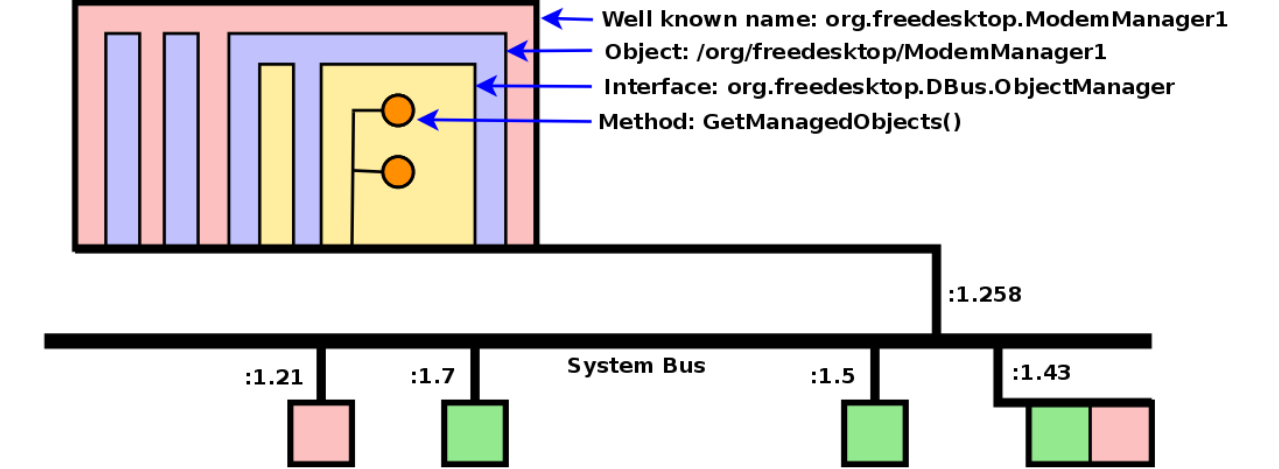
\includegraphics[width=0.6\linewidth]{dbus}}
\caption{Архитектура D-Bus}
\label{fig:dbus}
\end{figure}
\subsection{oFono}
Для организации общения с используемым sim-модулем был использолван программный проект oFono. Данный проект является бесплатным и распространяется под лицензией GNU GPL v2~\cite{oFono}. Проект oFono построен на стандарте 3GPP (3rg Generation Partnership Project) и использует D-Bus API для общения. Архитектура проекта oFono показана на рис. \ref{fig:ofono}.
\begin{figure}[H]
\center{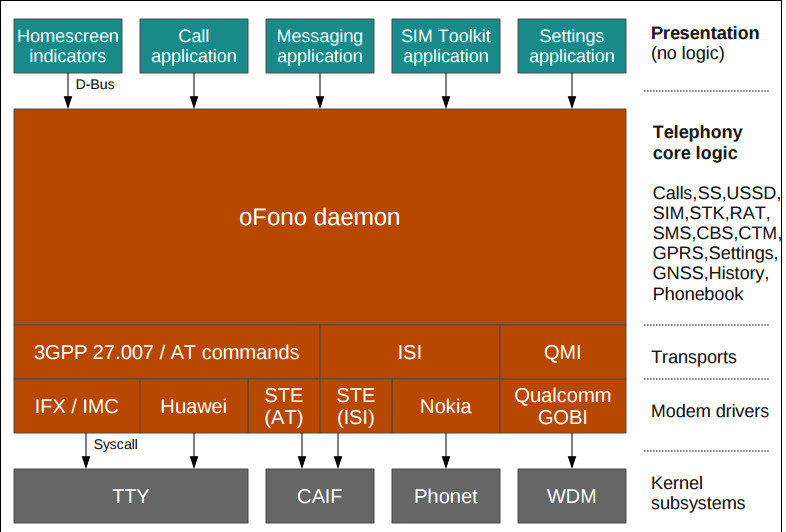
\includegraphics[width=0.6\linewidth]{ofono}}
\caption{Архитектура ofono}
\label{fig:ofono}
\end{figure}

Проект oFono был анонсирован компаниями Intel и Nokia в мая 2009 года. Последняя версия 1.4 была представлена в августе 2016 года. Работа над данным проектом ведется до сих пор. Исходные коды oFono находятся в свободном доступе, в гит репозитории~\cite{oFonoSources}.

Программный стек oFono поддерживает различные модули, такие как:
\begin{itemize}
\item 2G/3G
\item LTE
\item CDMA(Code-division multiple access)
\item GSM
\item Bluetooth и т.д.
\end{itemize}

Общаение между oFono и sim-модулем будет производится через различные AT-команды. В свою очередь, разрабатываемый демон будет общаться с oFono посредством D-Bus.

	\section{Анализ способов общения через D-Bus}
\subsection{QtDbus}
Qt --- это кросплатформенный инструментарий разработки программного обеспечения (ПО) на языке программирования \textit{C++}~\cite{Qt}. Qt позваляет запускать различные приложения, написанные с его помощью, на различных ОС, без необходимости переписывать исходный код. Одна из основных отличительных особенностей Qt - использование \textit{Meta Object Compiler (MOC)}. MOC - система предварительной обработки исходного кода. Она позволяет во много раз увеличить мощь библиотек вводя таки понятия, как \textit{слоты} и \textit{сигналы}. 

Qt позволяет создавать собственные плагины и размещать их непосредственно в панели визуального редактора. Также существует возможность расширения привычной функциональности виджетов, связанной с размещением их на экране, отображением, перерисовкой при изменении размеров окна.

Одним из весомых преимуществ проекта Qt является наличие качественной документации. Статьи документации снабжены большим количеством примеров. Исходный код самой библиотеки хорошо форматирован, подробно комментирован и легко читается, что также упрощает изучение Qt~\cite{QtDoc}.

Помимо <<чистого>> Qt, для реализации графического интерфейса можно использовать связку \textit{Qt + QML}. QML представляет из себя декларативный язык программирования, основанный на \textit{JavaScript}, предназначенный для создания дизайна приложений. QML документ выглядит как дерево элеиентов. Сам QML элемент представляет из себя совокупность блоков:
\begin{itemize}
\item Графических
	\begin{itemize}
	\item Rectangle
	\item Image и т.д.
	\end{itemize}
\item Поведенческих
	\begin{itemize}
	\item State
	\item Transition
	\item Animation и т.д.
	\end{itemize}
\end{itemize}

Qt обеспечивает возможностью работать с D-Bus через собственный модуль, который называется QtDBus. Данный модуль полностью инкапсулирует низкоуровневую концепцию обмена сообщений в более простую - объектно ориентированную модель. Для работы с данном модулем существует огромное количество классов, каждый из которых хорошо задокументирован.

\subsection{GLib}
GLib --- набор из низкоуровневых системных библиотек, написанных на языке программирования \textit{C} и разрабатываемых, в основном, \textit{GNOME}~\cite{gnome}. Исходные коды GLib были отделены от GTK+ и могут быть использованы ПО отличным от \textit{GNOME}. GLib распространяется под лицензией GNU GPL и исходные коды находятся на \textit{github}~\cite{glibSources}.

GLib предоставляет такие структуры данных, как:
\begin{itemize}
\item Одно- и двусвязные списки
\item Хэш-таблицы
\item Динамические массивы
\item Динамическиие строки
\item Сбалансированные двоичные деревья и т.д.
\end{itemize}




	\section{Выполнение работы}
\subsection{Описание тестового стенда}
Для выполнения работы использовалось два тестовых стенда:
\begin{itemize}
\item Платформа Raspberry Pi 1 с ОС ArchLinux и модуль SIM-808
\item Компьютер с ОС Ubuntu 16.04
\end{itemize}

В реальном стенде будет использована плата Raspberry Pi Zero и сим модуль SIM-808L. А благодаря тому, что модуль SIM-808 полностью совместим с модулем SIM-808L, то демон, который был разработан с использованием одного модуля будет совместим с другим модулем. Так как демон создавался независимым от реализации платформы, то не имеет особого значения, на какой ОС вести разработку.

\subsection{Выбор библиотеки}
Как было рассмотренно, для реализации общения по D-Bus существует несколько различных библиотек. Исходя из проведенного анализа, была выбрана библиотека \textit{dbus-glib} по той причине, что используемое устройствоя является маломощным, а так как у выбранной библиотеки малый уровень абстракции, то данный выбор позволяет нам увеличить производительность.

\subsection{Разработка демона}
Исходный код демона приведен в листинге \ref{lst:main}. В основной функции приложения main производятся следующие действия:
\begin{itemize}
\item Запись в лог информации о старте демона 
\item Подключение к системной шине D-Bus
\item Получение списка доступных модемов
\item Выбор модема
\item Попытка активации модема
\item Получение оператора
\end{itemize}

Парсинг полученного ответа и запись в лог-файл осуществляется с помощью заголовочного файла, код которого приведен в листинге \ref{lst:struct}. В данном заголовочном файле реализована структура, которая соответствует большинству ответов. В структуре два поля:
\begin{itemize}
\item Строка, соответствующая пути оьъекта (например, \textit{/sim900\_0} --- путь используемого модуля).
\item Словарь, который соответствует свойствам, где ключ - свойство, а значение - значение свойства.
\end{itemize}

Также, в демоне реализовано подключение к сигналу и его обработка. Далее будет подробнее рассмотрен этап подключения к сигналу.
\begin{itemize}
\item \textit{dbus\_error\_init} производит инициализацию структуры ошибки D-Bus.
\item \textit{dbus\_bus\_get} подключение к системной шине D-Bus.
\item \textit{dbus\_error\_is\_set} проверка на возникновение ошибки D-Bus.
\item \textit{dbus\_connection\_setup\_with\_g\_main} устанавливает функции наблюдения и тайм-аута DBusConnection для интеграции соединения с основным циклом.
\item \textit{dbus\_bus\_add\_match} добавляет правило соответствия для сообщений, проходящих через шину.
\item \texttt{dbus\_connection\_add\_filter} дообавляет фильтрпацию сообщений. Фильтры --- это обработчики сообщений, которые вызываются для обработки всех входящих сообщений, относящихся к зарегистрированному объекту. 
\end{itemize}

Помимо файла с исходным кодом и заголовочного файла, в структуру проекта входит \textit{CMakeLists} --- файл, предназначенный для сборки проекта. Содержание данного файла приведено в листинге \ref{lst:cmake}.

Пример исправной работы демона можно увидеть на рис. \ref{fig:daemon}

\begin{figure}
\center{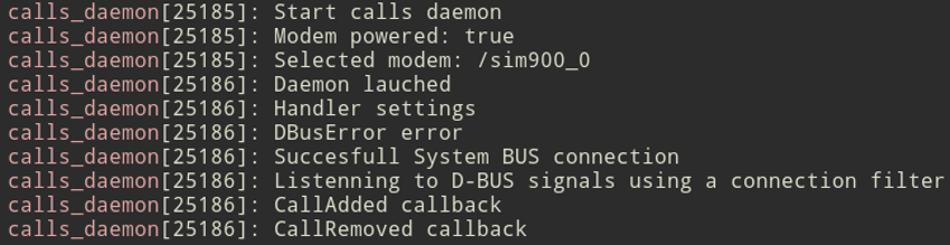
\includegraphics[width=0.6\linewidth]{daemon}}
\caption{Пример исправной работы демона}
\label{fig:daemon}
\end{figure}

\section{Дополнительная работа}
В ходе проекта, помимо создания демона звонков, была создана графическая оболочка для приложения телефона. В качестве платформы для создания графических приложений рассматривались две, одна из которых была описана выше, --- \textit{Qt} и \textit{GTK+}. В конечном итоге, была выбрана платформа Qt из-за того, что графика, написанная на \textit{Qt}, на конечной платформе выглядит приятнее, чем графика, написанная на \textit{GTK+}. 

Для создания графической оболочки была использована связка \textit{QT + QML}, а основная логика приложения --- \textit{C++}. Самым первым этапом создания основной логики приложения является создание самого приложения \textit{QApplication} (Листинг \ref{lst:mainqt}).
\begin{lstlisting}[label=lst:mainqt, caption={Создание приложения}]
int main(int argc, char *argv[])
{
	QApplication a(argc, argv);
	MainWindow w;
	return a.exec();
}
\end{lstlisting}
Класс \textit{MainWindow} представляет из себя основную логику графического окна. Реализация данного класса приведена в листингах~\ref{lst:mainwindowgui} --- \ref{lst:mainwindowh}. В данном классе выполняются следующия действия:
\begin{itemize}
\item Подключение к созданному приложению графической оболочки
\item Получение активированного модема
\item Совершение вызова
\item Завершение вызова
\end{itemize}

Для подключения графической состовляющей и различных изображений используются ресурсы. Использование ресурсов позволяет облегчить сборку приложения, тем самым, платформа нагружается немногим меньше, а время сборки уменьшается. Файл ресурсов выглядит следующим образом (листинг~\ref{lst:res}).
\begin{lstlisting}[label=lst:res, caption={Файл ресурсов}]
<RCC>
	<qresource prefix="/">
		<file>qml/main.qml</file>
		<file>qml/dialing.qml</file>
		<file>qml/core/Button.qml</file>
		<file>qml/call.qml</file>
		<file>pics/dial.png</file>
		<file>pics/erase.png</file>
		<file>pics/back.png</file>
		<file>pics/hang.png</file>
	</qresource>
</RCC>
\end{lstlisting}

Окна с графической реализацией имеют расширение \textit{.qml}. Главное окно и реализация класса \textit{Button} приведены в листингах~\ref{lst:mainqml}---\ref{lst:button}. Так как вместо стандартного класса \textit{Button} был использован свой класс, то приложению необходимо сообщить о том, что когда программист пытается реализовать класс \textit{Button}, вместо стандартного, нужно реализовывать созданный. Для этого нужна всего одна строчка в файле \textit{qmldir} (Листинг~\ref{lst:qmldir}).
\begin{lstlisting}[label=lst:qmldir, caption={Подключение класса Button}]
Button Button.qml
\end{lstlisting}

Для сборки проекта написанного на Qt принято использовать утилиту \textit{qmake}. Для ее использования создается файл с расширением \textit{.pro} и в него прописываются все зависимости. Используемый файл \textit{phone.pro} показан в листинге~\ref{lst:phone}.

Таким образом, было написано графическое приложение, позволяющее:
\begin{itemize}
\item Набирать номер
\item Совершать звонок
\item Отображать звонок
\item Сбрасывать звонок
\end{itemize}
Пример приложения приведен на рисунке~\ref{fig:phone}.
\begin{figure}
\center{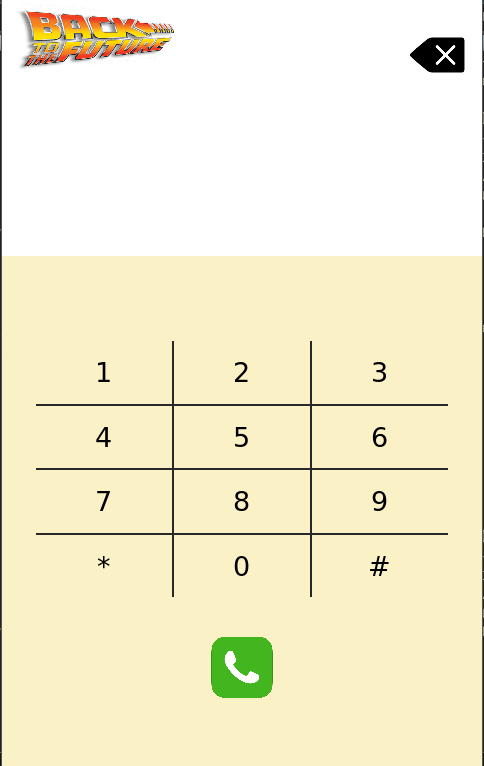
\includegraphics[width=0.6\linewidth]{phone}}
\caption{Пример работы графического приложения}
\label{fig:phone}
\end{figure}

	\section{Выводы}
В ходе работы были проанализированы и сравнены протоколы организации графических серверов в UNIX-подобных системах. В результате анализа было решено, что Wayland является более современной и оптимальной системой для разработки мобильного оконного менеджера.
В данной работе был реализован мобильный оконный менеджер для протокола Wayland. Данный оконный менеджер разрабатывался в рамках проекта по разработке мобильного телефона. Разработанный оконный менеджер позволяет запускать системные приложения (строка состояния и рабочий стол) и обычные пользовательские приложения. Оконный менеджер так же обрабатывает несколько комбинаций клавиш для управления окнами, а так же позволяет перемещать окна и изменять из размеры с помощью   мыши.
	\FloatBarrier
			
	\pagebreak
	\addcontentsline{toc}{section}{Список используемой литературы}
	\bibliography{biblio}
	\bibliographystyle{ugost2008}  %% стилевой файл для оформления по ГОСТу
	
	\pagebreak	
	\section{Прилагаемые материалы}
	Список прилагаемых материалов:
	\begin{itemize}
		\item Техническое задание.docx --- техническое задание на проект;
		\item progManual.pdf --- руководство системного программиста;
		\item sources.pdf --- текст программы;
		\item spec.pdf --- описание программы;
		\item tests.pdf --- программа и методика испытаний;
		\item userManual.pdf --- руководство пользователя.
	\end{itemize}
	
	
	\pagebreak
	\section*{Листинги}

\lstinputlisting[label=lst:main, caption={Файл main.c}, 
language={C}]{../src/main.c}

\lstinputlisting[label=lst:confh, caption={Файл config.h}, 
language={C}]{../src/config.h}

\lstinputlisting[label=lst:confc, caption={Файл config.c}, 
language={C}]{../src/config.c}

\lstinputlisting[label=lst:cmake, caption={Файл сборки CMakeLists.txt}, 
language={C}]{../src/CMakeLists.txt}
\end{document}
